\chapter{Hardware Configuration}
While the project is software heavy, the hardware to test the software must be correctly set up. This can helps frustration writing the software along the way.

\section{Schematic Diagram}
For this project these are the required hardware and materials:
\begin{itemize}
	\item Raspberry Pi
	\item SH1107
	\item TMP102
	\item Jumper wires
	\item Breadboard
\end{itemize}
SH1107 and  TMP102 are capable to communicate with Raspberry using I2C as interface and therefore can be connected parallel to each other. In Fig.~\ref{fig:fig1}, the data pin \verb'Pin 1' and clock pin \verb'Pin 2' from raspberry pi is connected both to data pin and clock pin respectively of both slave devices. VDD Pins must be connected to 3.3-volt power supply and GND pin to the Ground as usual. Additional Pin ADD0 from TMP102 may be connected to GND if standard address is chosen to be used, otherwise to the power supply.

\begin{figure}
	\centering
	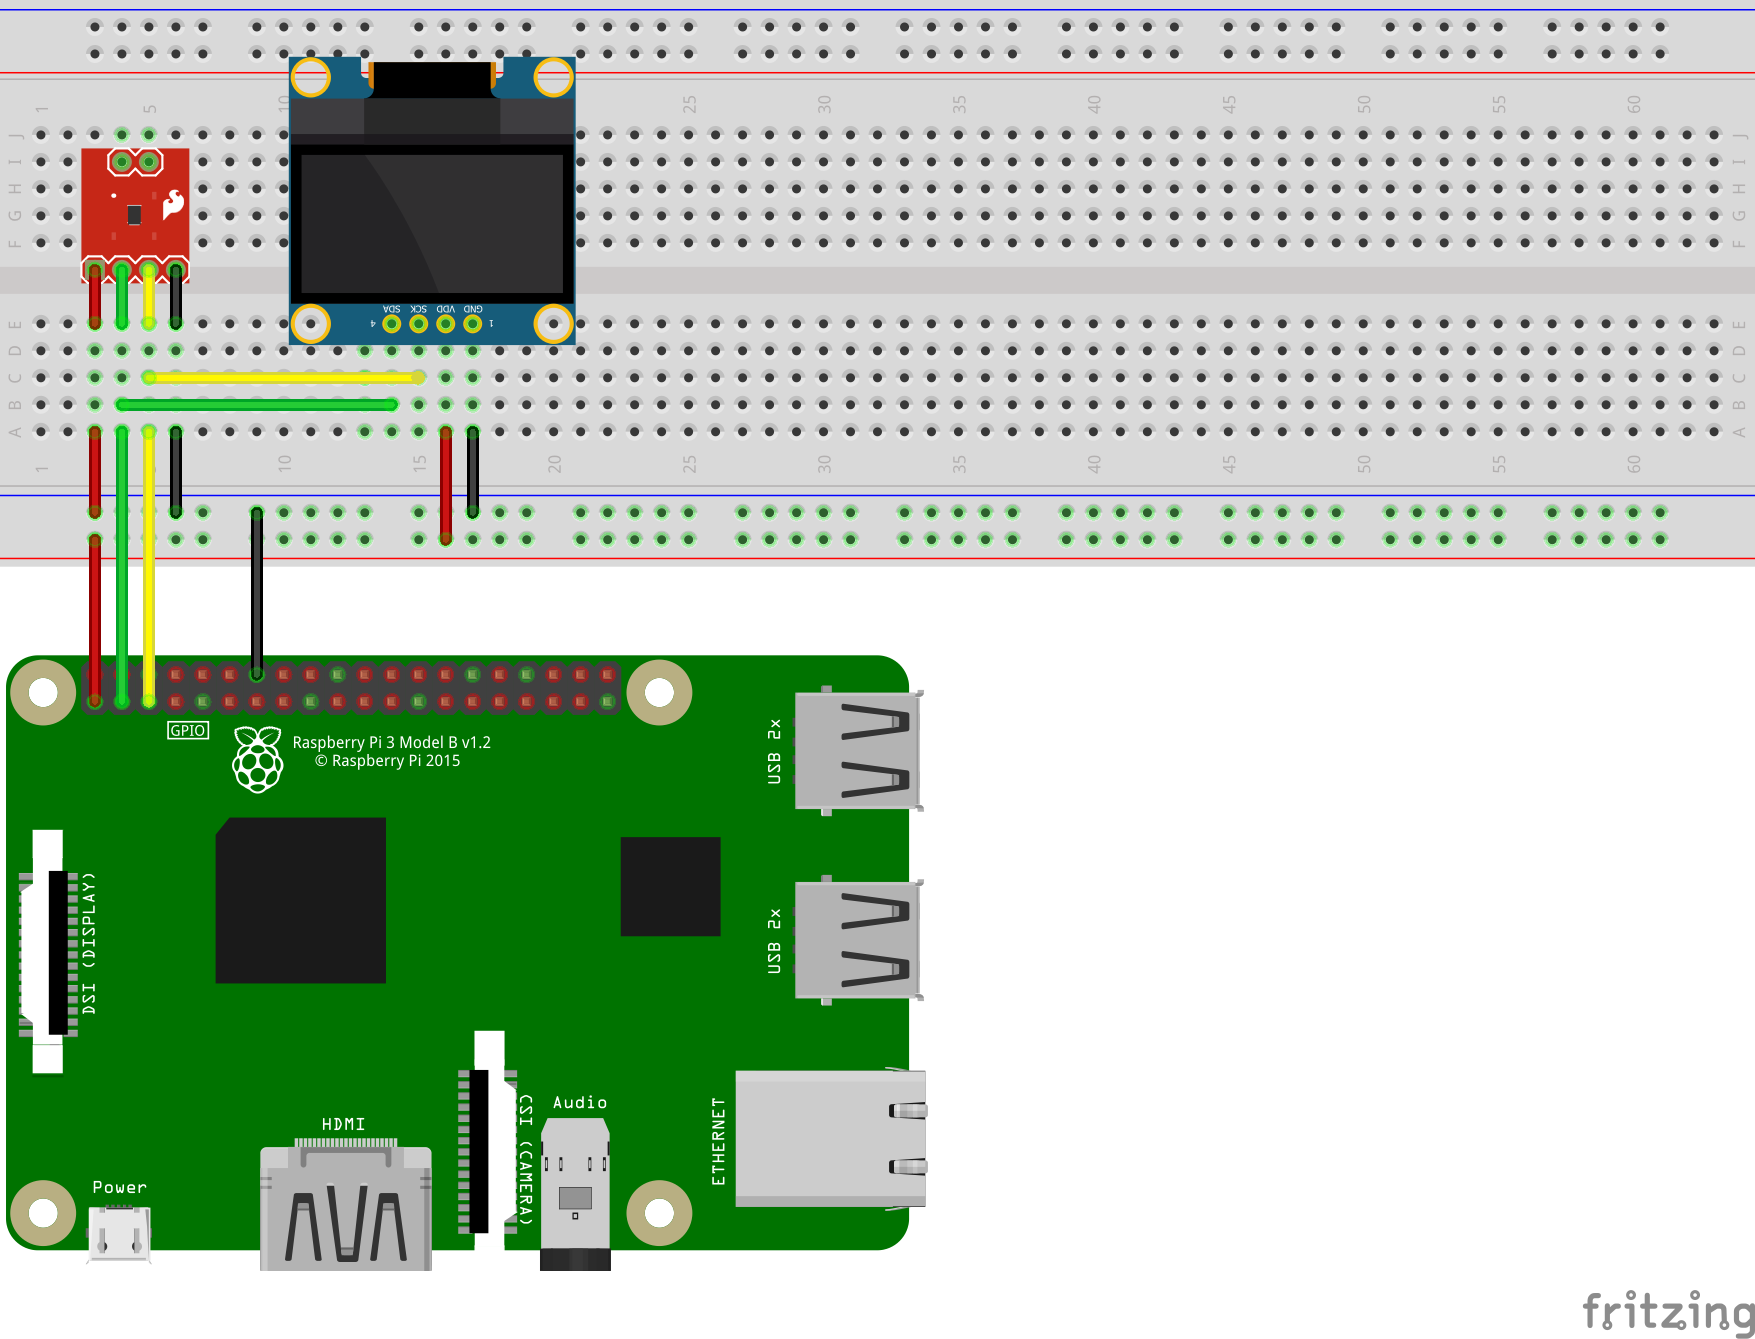
\includegraphics[width=.8\linewidth]{circuit-diagram.png}
	\caption{Circuit diagram for this project}\label{fig:fig1}
\end{figure}

\section{I2C-bus Interface}
I2C (Inter-Integrated Circuit) is a widely used serial communication protocol designed for efficient data transfer between electronic devices. It was developed by Philips (now NXP Semiconductors) and is now an industry standard~\cite{noauthor_i2c-bus_2021}
. The I2C protocol utilizes a master-slave architecture, where a master device initiates communication and controls the data flow, while the slave devices respond to the master's requests. Communication occurs over two lines: a clock line (SCL) and a data line (SDA). The clock line synchronizes the data transfer, while the data line carries the actual information. The I2C protocol supports multiple devices connected to the same bus, each identified by a unique address~\cite{valdez_understanding_2015}
. This allows for easy integration of various components such as sensors, memory chips, and displays into a system. With its simplicity, versatility, and wide support across different microcontrollers and peripherals, I2C has become a popular choice for interconnecting devices in applications ranging from consumer electronics to industrial systems.

Fig.~\ref{fig:fig2} represent a complete data transfer from one device to another~\cite{noauthor_i2c-bus_2021}
. All of I2C components should send data according to the mentioned interface. The I2C-bus is for bi-directional, two-line communication between different ICs or modules. The two lines are a serial data line (SDA) and a serial clock line (SCL). Both lines must be connected to a positive supply via a pull-up resistor. Data transfer may be initiated only when the bus is not busy. Therefore, there are several steps must be followed to avoid concurrent of data among the devices. These process algorithm can be represented as followings~\cite{mankar2014review}
:
\begin{enumerate}
	\item Master Issue START conditions
	\item Slave device get ready
	\item Mater sends the ADDRESS of the device along with access whether read or write
	\item All ICs compare the address with its own
	\item If it does not match, it waits for stop bit
	\item If it matches, it will send an ACK signal
	\item Master receives the ACK signal and start transmitting and receiving data 
	\item Master issue STOP condition
\end{enumerate}

\begin{figure}
	\centering
	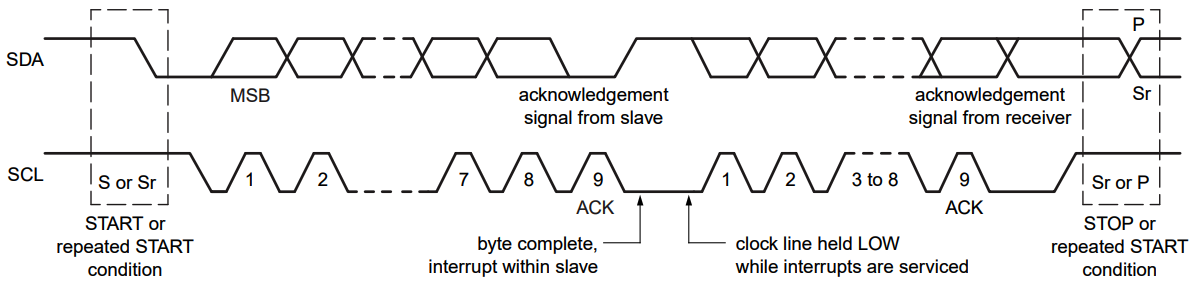
\includegraphics[width=.8\linewidth]{I2CInterface.png}
	\caption{I2C Data Signal with Clock Signal}\label{fig:fig2}
\end{figure}

\section{TMP102}
The TMP102 is a popular digital temperature sensor widely used in various applications. Developed by Texas Instruments, the TMP102 offers high accuracy and low power consumption, making it suitable for both battery-powered devices and industrial systems. This sensor operates over a wide temperature range, typically from -40°C to 120°C, with a resolution of 0.0625°C. It communicates with the raspberry pi through an I2C interface, allowing for easy integration into existing systems. With its compact size and straightforward operation, the TMP102 has become a reliable choice for temperature monitoring in a diverse range of applications, including automotive, consumer electronics, and environmental monitoring systems~\cite{TMP102_datasheet}
.

The data read from the sensor is in binary and therefore must be converted beforehand to be used as degree °C. Followings are the method to convert hex to degree celsius.

\begin{enumerate}
	\item Convert the 12-bit, left-justified binary temperature result, with the MSB = 0 to denote a positive sign, to a decimal number.
	\item Multiply the decimal number by the resolution to obtain the positive temperature.
	\item Example: 0011 0010 0000 = 320h = 800 × (0.0625°C / LSB) = 50°C
\end{enumerate}

\section{SH1107}
The SH1107 is a popular OLED (Organic Light-Emitting Diode) display controller designed for small-size displays. 
Developed by Solomon Systech Limited, the SH1107 offers a compact and efficient solution for driving monochrome OLED panels. 
With its built-in display RAM, the SH1107 enables fast and seamless rendering of graphics and text on the OLED screen. 
The controller communicates with a microcontroller or other host device through an I2C or SPI interface, providing flexibility in system integration. 
The SH1107 also incorporates advanced features such as screen scrolling, contrast control, and a built-in charge pump for generating the required OLED supply voltage. 
Due to its compact size, low power consumption, and versatile capabilities, the SH1107 has gained popularity in various applications, including wearable devices, portable gadgets, and small-scale IoT (Internet of Things) projects. \cite{SH1107_datasheet}

SH1107 differentiate whether the bytes received from Master is data or commands. When the D/Csharp pin is low, the data sent is interpreted as a command. When it is high, the data sent is treated as display data. These followings steps can be taken to configure and write data into SH1107:

\subsection{Initialization}
To initialize the SH1107 controller, specific initialization commands are sent. These commands typically include display configuration settings such as display resolution, multiplex ratio, display offset, and display start line. Additionally, you may need to set the segment remap and common output scan direction to configure the display orientation.

\subsection{Display Control}
The SH1107 offers commands to control the display behavior. These commands include turning the display on or off, setting the display contrast, and inverting the display colors. You can use these commands to adjust the appearance and visibility of the content on the OLED screen.

\subsection{Memory Addressing}
The SH1107 has a display memory that stores the pixel data for the OLED panel. The controller provides commands to set the memory addressing mode. This allows you to choose the addressing mode that suits your specific application requirements, such as horizontal or vertical addressing.

\subsection{Data Writing}
To draw graphics and write text on the display, you need to send the pixel data to the SH1107 controller. The pixel data is typically sent in a sequential manner, following the configured addressing mode. By providing the appropriate pixel data to the controller, you can control the appearance of the content displayed on the OLED screen.

